\section{Operating principles}

Having successfully constructed the DNA nanopiston, now the operation cycle can be
discussed. For convenience, we take the rotaxane-ds configuration as the starting point
of this cycle. The power stroke of the molecular machine is initiated by bringing ssDNA
$4$ $(0.5\ \mu M)$ into solution at the tran-side. This strand is fully complementary to
ssDNA $2$, thereby inducing a toehold-mediated strand displacement. Here the
flexible overhang located at the end of ssDNA $2$, referred to as the toehold, is used to
mediate the hybridisation of ssDNA $2$ and $4$ (Fig ..).

During the strand displacement reaction, two possible transient states can possibly
occur. On of the possibly scenario's describes the hybridisation happening inside of the
nanopore. This scenario is deemed to be unlikely since this process would require three
strands of ssDNA to be simultaneously present inside the constriction of the nanopore.
Alternatively, the hybridisation can take place outside of the nanopore, in the
trans-side of the reservoir. This process implies that the neutravidin protein would
enter the lumen of the pore, which has been showed by previous studies to be possible.
This second scenario is thereby thought of as the most probable.

The resulting configuration of this process is called the rotaxane-ds in view of the fact
that the state is predominately composed of ssDNA.


The subsequent addition of 0.5 μM ofssDNA 2 cargo to the cis side restores rotaxane-ds,
as ssDNA 2 hybridizes with the thread of rotaxane-ss

After each cycle, one cargo molecule is transported from cis to trans and one fuel
molecule is expended.

These cycles were found to be both at positive, + 20 mV (Figure 2a, top trace), + 50 mV
and +100 mV (Figure S3), and negative, − 20 mV (Figure 2a,
bottom trace), biases. Higher negative applied potentials (e.g., −50 mV, Figure S3)
prevented the cycling

The working of the nanopiston against and with external bias is important, postulated
that it is due to the entropic interaction between the rotaxane and the pore.
Discuss the importance of entropy. power stroke is toehold disp reaction. Results in lwo
entropy state. This entropic energy provides the recovery stroke. Next hybridisation with
the fuel strand makes us come back to the intial configuration.

Furthermore, the cycles were faster at positive than at negative applied potentials, but
were slower as the potential was increased. This voltage dependency can be explained by
toehold sequestering inside the nanopore

% Due to brownian motion both autonomous and non-autonomous systems use ratcheting to
% eventually deliver work. Using this method minimal synthetic machines can deliver
% elegance and performance shedding the 'baggage' of biological evolution.

Figure 2.2a shows the measured current over through the nanopore during the operation
cycle. The ionic current of rotaxane-ss is lower than the blocked current ofrotaxane-ds
most likely reflecting the coiled structure of ssDNA inside the nanopore. Shows the
limitation of the experimental analysis of the pore, only view into the system is
throught the measured current. To get a more indepth understanding of the conformal
fluctuations of the pore computation analysis was performed in the form of molecular
dynamics simulations.


% Dit nog ergens bij schrijven idk waar, maar deze krachten zijn wel belangrijk?
% misschien bij de biological nanopores.
% Electrophoretic, electro-osmotic and entropic forces are, in principle, acting on the
% rotaxanes. The electrophoretic force sets the negatively charged DNA in motion, under the
% action of the applied bias (from cis to trans for
% ∆?? > 0 ). Electroosmosis generates an opposing force, arising from the motion of cations
% accumulated on the walls of the negatively charged ClyA pore and the DNA thread. Finally,
% the entropic force is solely geometry specific, and pushes the rotaxane towards
% conformations with high configurational entropy. Entropic forces are expected to play an
% important role in the rotaxanes studied here, which are composed of stiff dsDNA and
% flexible ssDNA parts.



\begin{figure}[ht]
  \begin{centering}
  \adjustbox{minipage=1.3em,valign=t}{\subcaption{}\label{sfig:testa}}%
  \begin{subfigure}[t]{\dimexpr.95\linewidth-1.3em\relax}
  \centering
  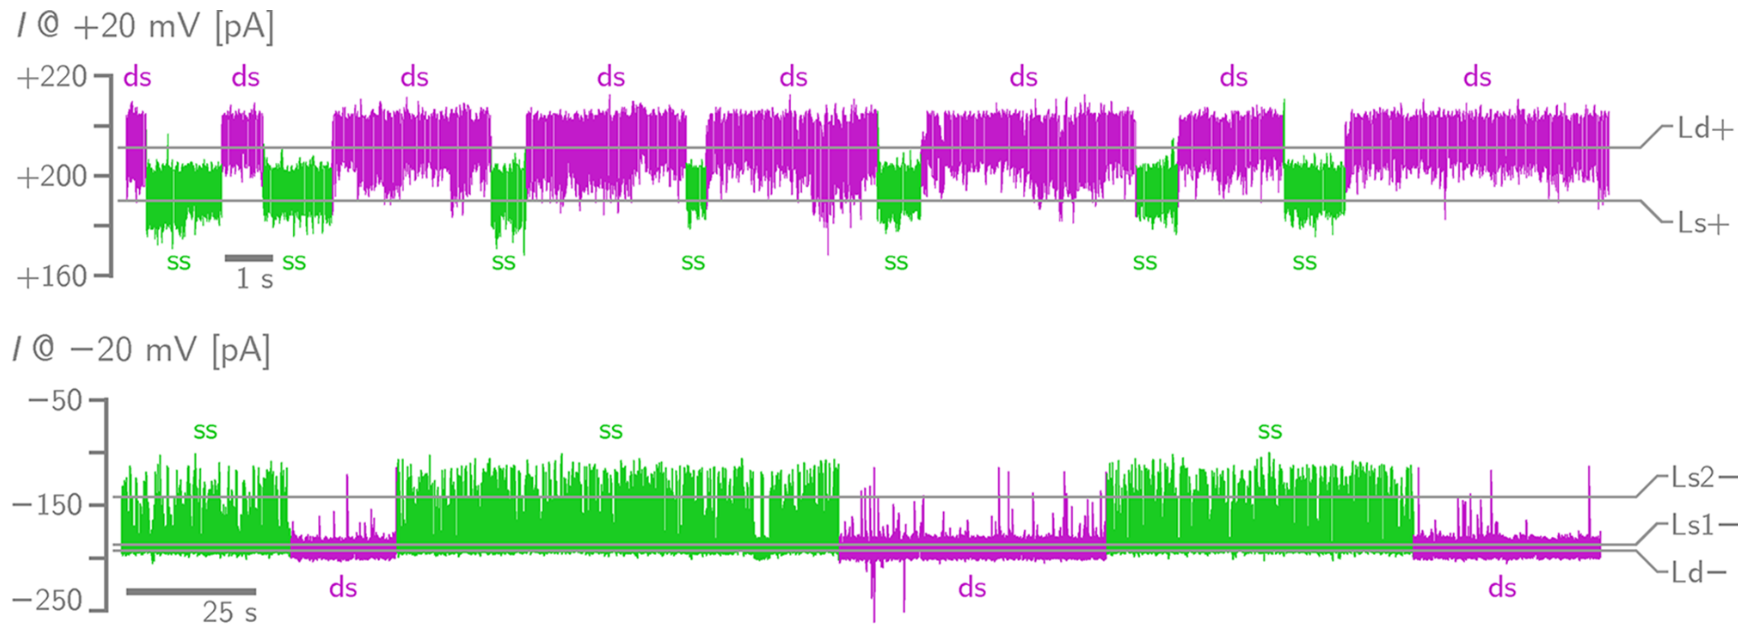
\includegraphics[width=\linewidth,valign=t]{Figures/FluctuationRotaxane.png}
  \end{subfigure}%
  \vspace{0.5cm}
  \adjustbox{minipage=1.3em,valign=t}{\subcaption{}\label{sfig:testb}}%
  \begin{subfigure}[t]{\dimexpr.5\linewidth-1.3em\relax}
  \centering
  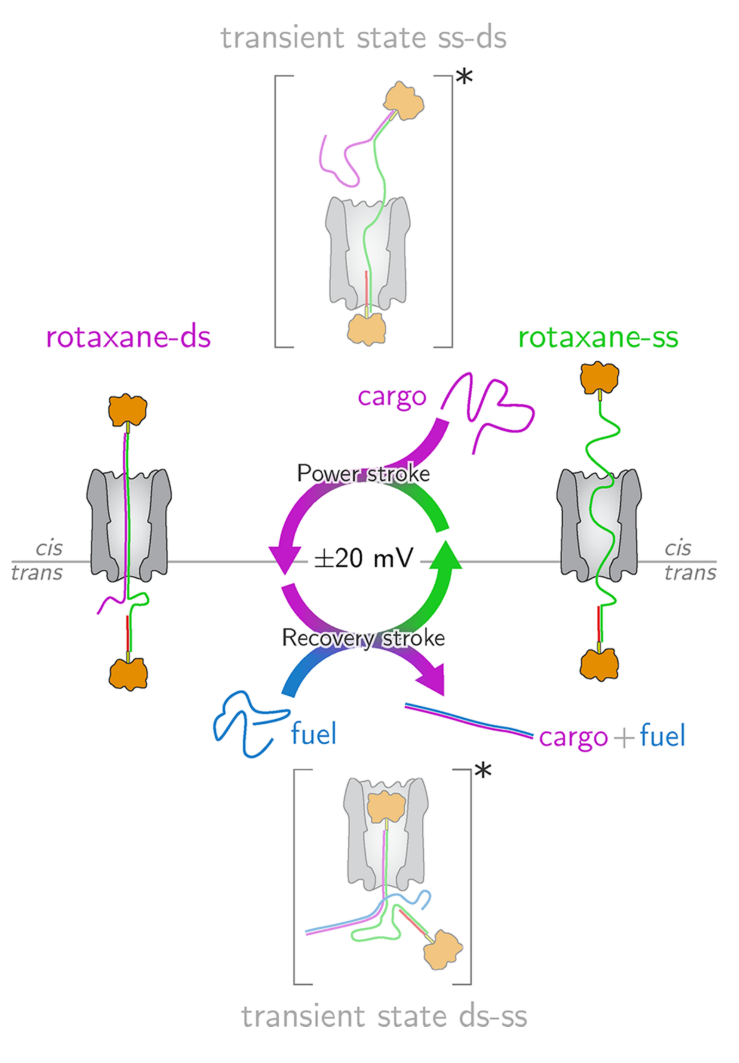
\includegraphics[width=\linewidth,valign=t]{Figures/RotaxaneCycle.png}
  \end{subfigure}
  \caption{This is a figure}
  \label{fig:test}
  \end{centering}
\end{figure}
